\section{Code verification}
The verification was done by checking if the output of the function (\texttt{c} and \texttt{alfaHat}) matches the given values of \texttt{c} and \texttt{alfaHat} for the example given in section A.3 of the Exercise Project (page 238). The corrected code passed the test case.

We identified the following errors:

\large{1}\\
\textbf{Original}: \texttt{T = size(pX)}\\
\textbf{Corrected}: \texttt{T = size(pX, 2)}\\
\textbf{Type of flaw}: Logical and Runtime\\
\textbf{Comments}: T is duration of the observed pattern sequence and hence it is a scalar value and not a vector.

\large{2}\\
\textbf{Original}: \texttt{alfaTemp = zeros(numberOfStates);}\\
\textbf{Corrected}: \texttt{alfaTemp = zeros(numberOfStates, 1);}\\
\textbf{Type of flaw}: Logical\\
\textbf{Comments}: alfaTemp is a temporary value should get reset after calculating alfaHat for every time step 't'. Also, since it is reset everytime it will be a row vector with number of states as its size. Without this correction, we get incorrect dimensions of alfaHat and hence alfaHat in general becomes incorrect.

\large{3}\\
\textbf{Original}: \texttt{alfaTemp(j) = alfaTemp(j)/c(2)}\\
\textbf{Corrected}: \texttt{alfaTemp(j) = alfaTemp(j)/c(t,1);}\\
\textbf{Type of flaw}: Logical\\
\textbf{Comments}: Incorrect c and alfaHat values and dimension. alfaTemp has to be normalised with c at that time instance 't'. This is because, alfaHat for a time instance 't' is the normalized state probabilities given the observations at the time instance 't'.

\large{4}\\
\textbf{Original}: \texttt{alfaHat = [alfaHat alfaTemp']}\\
\textbf{Corrected}: \texttt{alfaHat = [alfaHat alfaTemp]}\\
\textbf{Type of flaw}: Runtime\\
\textbf{Comments}: Error : Dimensions of matrices being concatenated are not consistent.

\large{5}\\
\textbf{Original}: \texttt{c(max(rows,columns)) = 0.0581]}\\
\textbf{Corrected}: \texttt{c(max(rows,columns)+1) = 0.0581}\\
\textbf{Type of flaw}: Logical\\
\textbf{Comments}: For a finite duration HMM, we need to include the special exit condition $S_{(T+1)}$  and hence the exit probability is is for $c_{(T+1)}$.

\large{6}\\
\textbf{Original}: \texttt{c(max(rows,columns)+1) = 0.0581;}\\
\textbf{Corrected}: \texttt{c(max(rows,columns)+1) = alfaTemp'*A(:,columns);}\\
\textbf{Type of flaw}: Logical\\
\textbf{Comments}: The value is hardcoded (and thus passes the tests) instead of calculated.

\section{Character database}
We have added the following 15 characters to our training dataset: A, B, C, i, O, Q, T, U, V, W, 1, 2, 4, ! and +.

For each character, we made 15 samples so we have a total of 225 samples.

\section{Why these characters?}
We chose these characters for the following reasons:
\begin{itemize}
\item A, B and C simply because they are the first three characters.
\item T and + because they are specifically mentioned in one of the previous exercises as difficult to distinguish.
\item C, O and Q because the "roundish" shape looks visually similar, but they have some small differences (not a full circle for the C, and an extra line for the Q).
\item U, V and W because they are somewhat similar in shape too, especially U and V.
\item i and ! because the basic shapes are the same (a line and a dot); only the relative position of the dot distinguishes the two.
\item 1, 2 and 4 for the sake of having some numbers too. Also, the 1 (being a single line) is similar to the ! and i but doesn't have the dot.
\end{itemize}

\subsection{Variations in characters}
For each character, we used the same drawing movements. For example; when drawing a "T", we first draw a line from the left to the right (the top line) and then a line from the centre top to the bottom.

We only varied angles, drawing speed, size and position (offset) of the characters. We think that this should be sufficient for recognizing one persons handwriting.

Most people will draw a C starting at the top, and ending at the bottom. Of course, it would be totally possible to train our HMM on the reverse movement too (it should result in the same figure), but we don't think it's likely anyone draws it that way.

To visualize the differences in drawing one character repeatedly, we include the following three graphs. Each graph shows the direction element 

\begin{figure}[H]
	\centering
	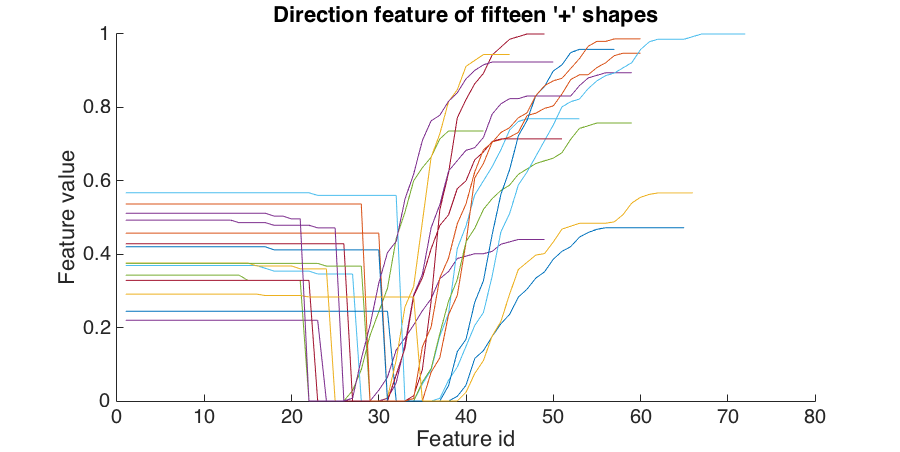
\includegraphics[width=.95\linewidth]{images/direction_plots_+}
	\captionof{figure}{Direction vector of fifteen drawings of '+'}
\end{figure}

\begin{figure}[H]
	\centering
	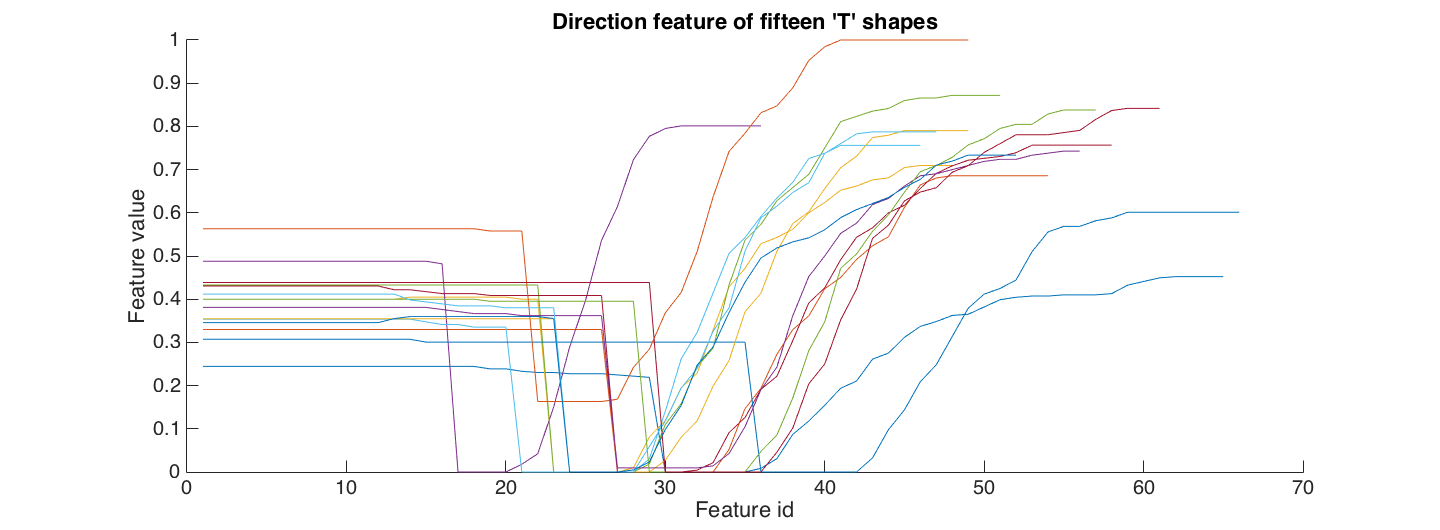
\includegraphics[width=.95\linewidth]{images/direction_plots_T}
	\captionof{figure}{Direction vector of fifteen drawings of 'T'}
\end{figure}

\begin{figure}[H]
	\centering
	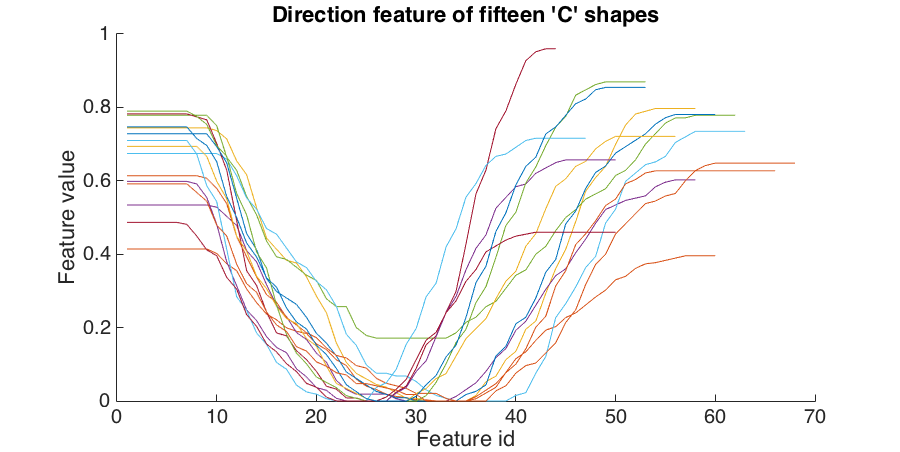
\includegraphics[width=.95\linewidth]{images/direction_plots_C}
	\captionof{figure}{Direction vector of fifteen drawings of 'C'}
\end{figure}